\documentclass{beamer}
\usepackage[UTF8]{ctex}
\usepackage{ulem}
\usepackage{amsmath}
\usepackage{amssymb}
\usepackage{geometry}
\usepackage{graphicx}  
\usepackage{subfigure}  
\usepackage{fancyhdr}
\usepackage{listings}
\usepackage{color}
\usepackage{pfnote}
\usepackage{listings}
\usepackage{xcolor}
\usepackage{cite}
\usetheme{CambridgeUS}
\usecolortheme{dolphin}

% 下面的内容会在标题页上展示
\title{OI数据结构之树状数组}

\author{GzsJAY\underline Official \and 有为骚年}
\institute{HI-OIER}
\date{August, 2025}

\begin{document}% 下面都是要显示的内容
	\frame{\titlepage}% 显示标题页
	
	\begin{frame}
		\frametitle{关于我}
		我是2011年出生的究极无敌蒟蒻 \\
		天天被 5033 ls 和 jzc ls单调队列 \\
		被chennie ls + karma ls吊打 \\
		入坑OI一年半的新玩家 \\
		希望混E类省队的究极大菜鸡 \\
		
		联系方式 
		QQ:3224063731(备注B站算法) 否则不认识QAQ
		\tableofcontents
	\end{frame}
	
	\begin{frame}
		\frametitle{树状数组是什么?}
			树状数组是一种支持“单点修改,区间查询”/“区间修改,区间查询” \\
			\pause
			它是通过什么实现的? \\
			\pause
			通过位运算(lowbit)存储位置,实现O(log n)的时间复杂度 \\
			\pause
			\begin{figure}
				\centering
				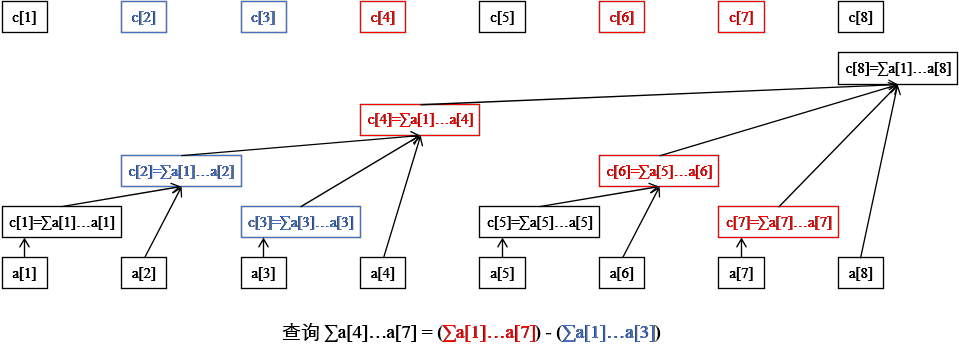
\includegraphics[width=0.7\linewidth]{pic/BIT}
				\caption{}
				\label{fig:bit}
			\end{figure}
			\pause
			你发现了什么?\\
	\end{frame}
	
	\begin{frame}
		\frametitle{树状数组的工作原理}
		树状数组实际上并不是一棵树 \\
		\begin{figure}
			\centering
			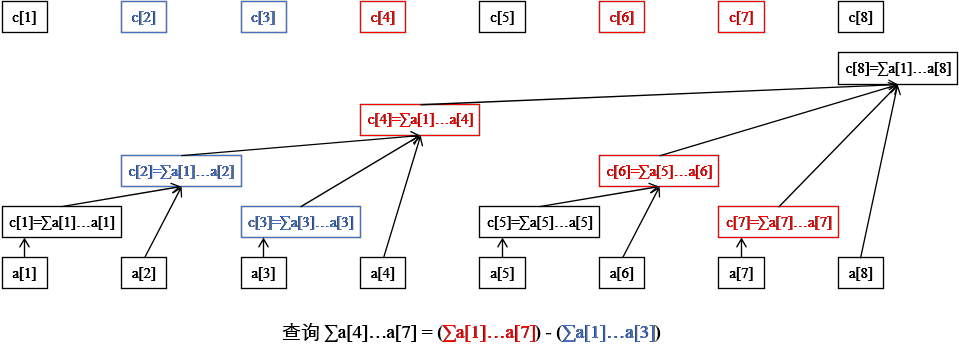
\includegraphics[width=0.7\linewidth]{pic/BIT}
			\caption{}
			\label{fig:bit}
		\end{figure}
		\pause
		从这张图片里我们可以观察到,$C_i$ 为 $a_?$ 到 $a_i$ 的和。 \\
		\pause
		这时你可能要说了,UP,那我们是不是可以用区间和了?
	\end{frame}
	
	\begin{frame}
		\frametitle{树状数组的工作原理}
				\begin{figure}
			\centering
			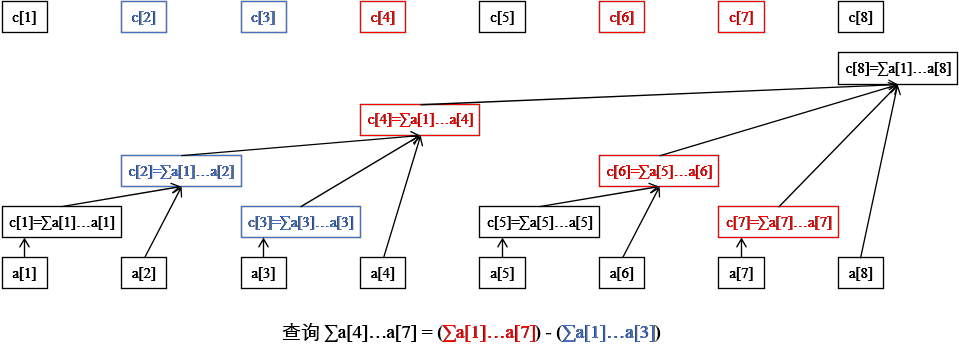
\includegraphics[width=0.7\linewidth]{pic/BIT}
			\caption{}
			\label{fig:bit}
		\end{figure}
		没错!但是我们该如何维护数组C呢? \\
	\end{frame}
	
	\begin{frame}
		\frametitle{lowbit}
		这个时候就应该聊到开头的lowbit了,\\
		\pause
		lowbit 的实质是将一个数的二进制全部取反 即\\
		\lstinline|int lowbit(int x) { return x & -x; }| \\
		\pause
		这对我们的树状数组有什么用呢?\\
		\pause
		很显然,可以用来求 $h_i$ 中 $i$ 的值 \\
		\pause
		联系之前提到的图片,我们可以发现,$C_i$ 管辖的区间为 $a[x-lowbit(x)+1, x]$
	
	\end{frame}
	
	\begin{frame}
		\frametitle{实现前缀和}
		首先实现前缀和 \\
		\pause
		根据刚刚的结论,即 $C_i$ 管辖的区间为 $a[x-lowbit(x)+1, x]$ \\
		可以得出实现求前缀和的代码 \\ 
		即 \\ 
		\begin{figure}
			\centering
			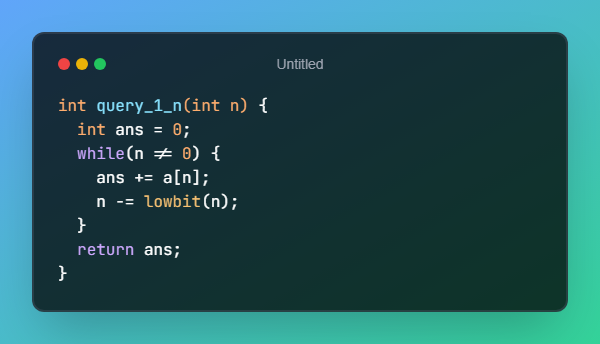
\includegraphics[width=0.7\linewidth]{pic/query_1_n}
			\caption{}
			\label{fig:query1n}
		\end{figure}
	\end{frame}
	
	\begin{frame}
		\frametitle{实现区间和}
		有了前缀和,区间和也很好求了。 \\
		\pause
		就是用 $A_1$ 到 $A_R$ 的前缀和 减去 $A_1$ 到 $A_L$ 的前缀和 (记得L区间-1)
		\pause
		实现代码
		\begin{figure}
			\centering
			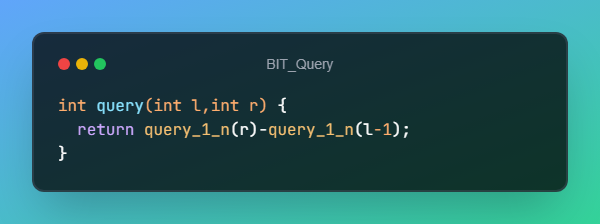
\includegraphics[width=0.7\linewidth]{pic/query}
			\caption{}
			\label{fig:query}
		\end{figure}
	\end{frame}
	
	\begin{frame}
		\frametitle{实现单点修改}
		既然我们的C数组是像下图一样实现的 \\
		\begin{figure}
			\centering
			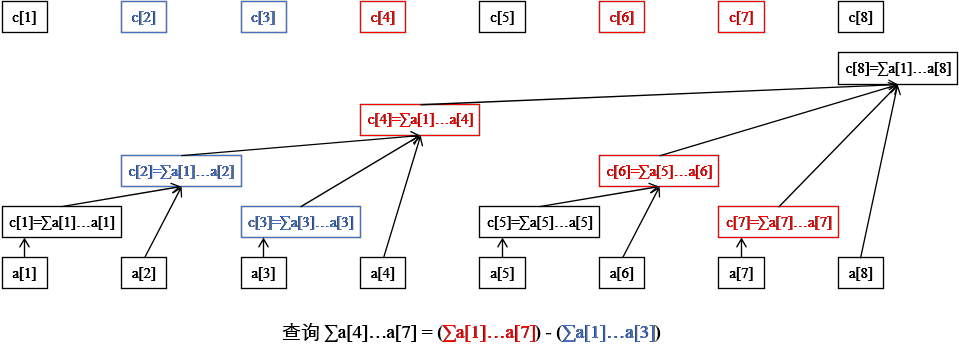
\includegraphics[width=0.7\linewidth]{pic/BIT}
			\caption{}
			\label{fig:bit}
		\end{figure}
		那么就可以很自然的知道,修改一个值,要把那个值的父亲节点也给同步更新了 \\
		实现也很简单
		\pause
	\end{frame}
	
	\begin{frame}
		\frametitle{实现单点修改}
		\begin{figure}
			\centering
			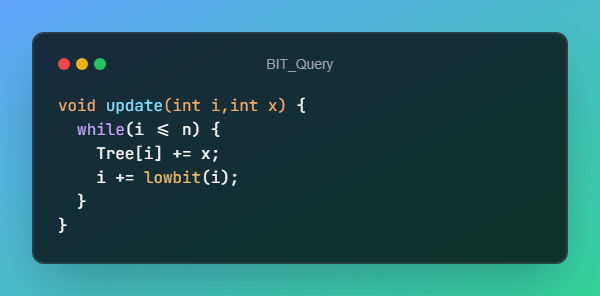
\includegraphics[width=0.7\linewidth]{pic/update}
			\caption{}
			\label{fig:update}
		\end{figure}
	\end{frame}	
	
	\begin{frame}
		\frametitle{最后}
		最后,我把代码模板和讲义放到了我的GitHUB仓库里,欢迎大家来查看(白嫖) \\
		最后的最后,再给大家推荐几道树状数组的题目 \\
		
		https://www.luogu.com.cn/problem/P3374 板子\\
		https://codeforces.com/contest/2130/problem/D 很经典的逆序对用法
	\end{frame}

\end{document}